\documentclass[tikz,border=10pt]{standalone}
\usepackage[T1]{fontenc}
\usepackage{lmodern}
\usetikzlibrary{arrows.meta,backgrounds,positioning,shapes.geometric}

\definecolor{ink}{HTML}{172033}
\definecolor{muted}{HTML}{59697F}
\definecolor{panel}{HTML}{F8FAFC}
\definecolor{panelborder}{HTML}{DCE5F0}
\definecolor{purple}{HTML}{7138E8}
\definecolor{purplefill}{HTML}{F0ECFF}
\definecolor{blue}{HTML}{2563EB}
\definecolor{bluefill}{HTML}{E1EDFF}
\definecolor{green}{HTML}{169B45}
\definecolor{greenfill}{HTML}{E1FBEA}
\definecolor{amber}{HTML}{D97706}
\definecolor{amberfill}{HTML}{FFF3C4}

\tikzset{
  flow/.style={
    -{Latex[length=2.7mm,width=2.1mm]},
    draw=muted,
    line width=1.05pt,
    rounded corners=3pt
  },
  agent/.style={
    draw=purple,
    fill=purplefill,
    line width=1.1pt,
    rounded corners=4pt,
    minimum width=38mm,
    minimum height=14mm,
    align=center,
    inner sep=3pt
  },
  tool/.style={
    draw=blue,
    fill=bluefill,
    line width=1.1pt,
    rounded corners=4pt,
    minimum width=42mm,
    minimum height=14mm,
    align=center,
    inner sep=3pt
  },
  passive/.style={
    draw=green,
    fill=greenfill,
    line width=1.1pt,
    rounded corners=4pt,
    minimum width=39mm,
    minimum height=14mm,
    align=center,
    inner sep=3pt
  },
  decision/.style={
    diamond,
    aspect=1.6,
    draw=amber,
    fill=amberfill,
    line width=1.1pt,
    minimum width=27mm,
    minimum height=17mm,
    align=center,
    inner sep=1pt
  },
  edge label/.style={
    fill=panel,
    inner sep=2pt,
    font=\sffamily\bfseries\small,
    text=muted
  },
  note/.style={
    fill=greenfill,
    rounded corners=5pt,
    inner xsep=7pt,
    inner ysep=3.5pt,
    font=\sffamily\bfseries\small,
    text=green
  },
  loop note/.style={
    draw=purple,
    fill=purplefill,
    line width=0.8pt,
    rounded corners=5pt,
    inner xsep=7pt,
    inner ysep=3.5pt,
    font=\sffamily\bfseries\small,
    text=purple
  }
}

\begin{document}
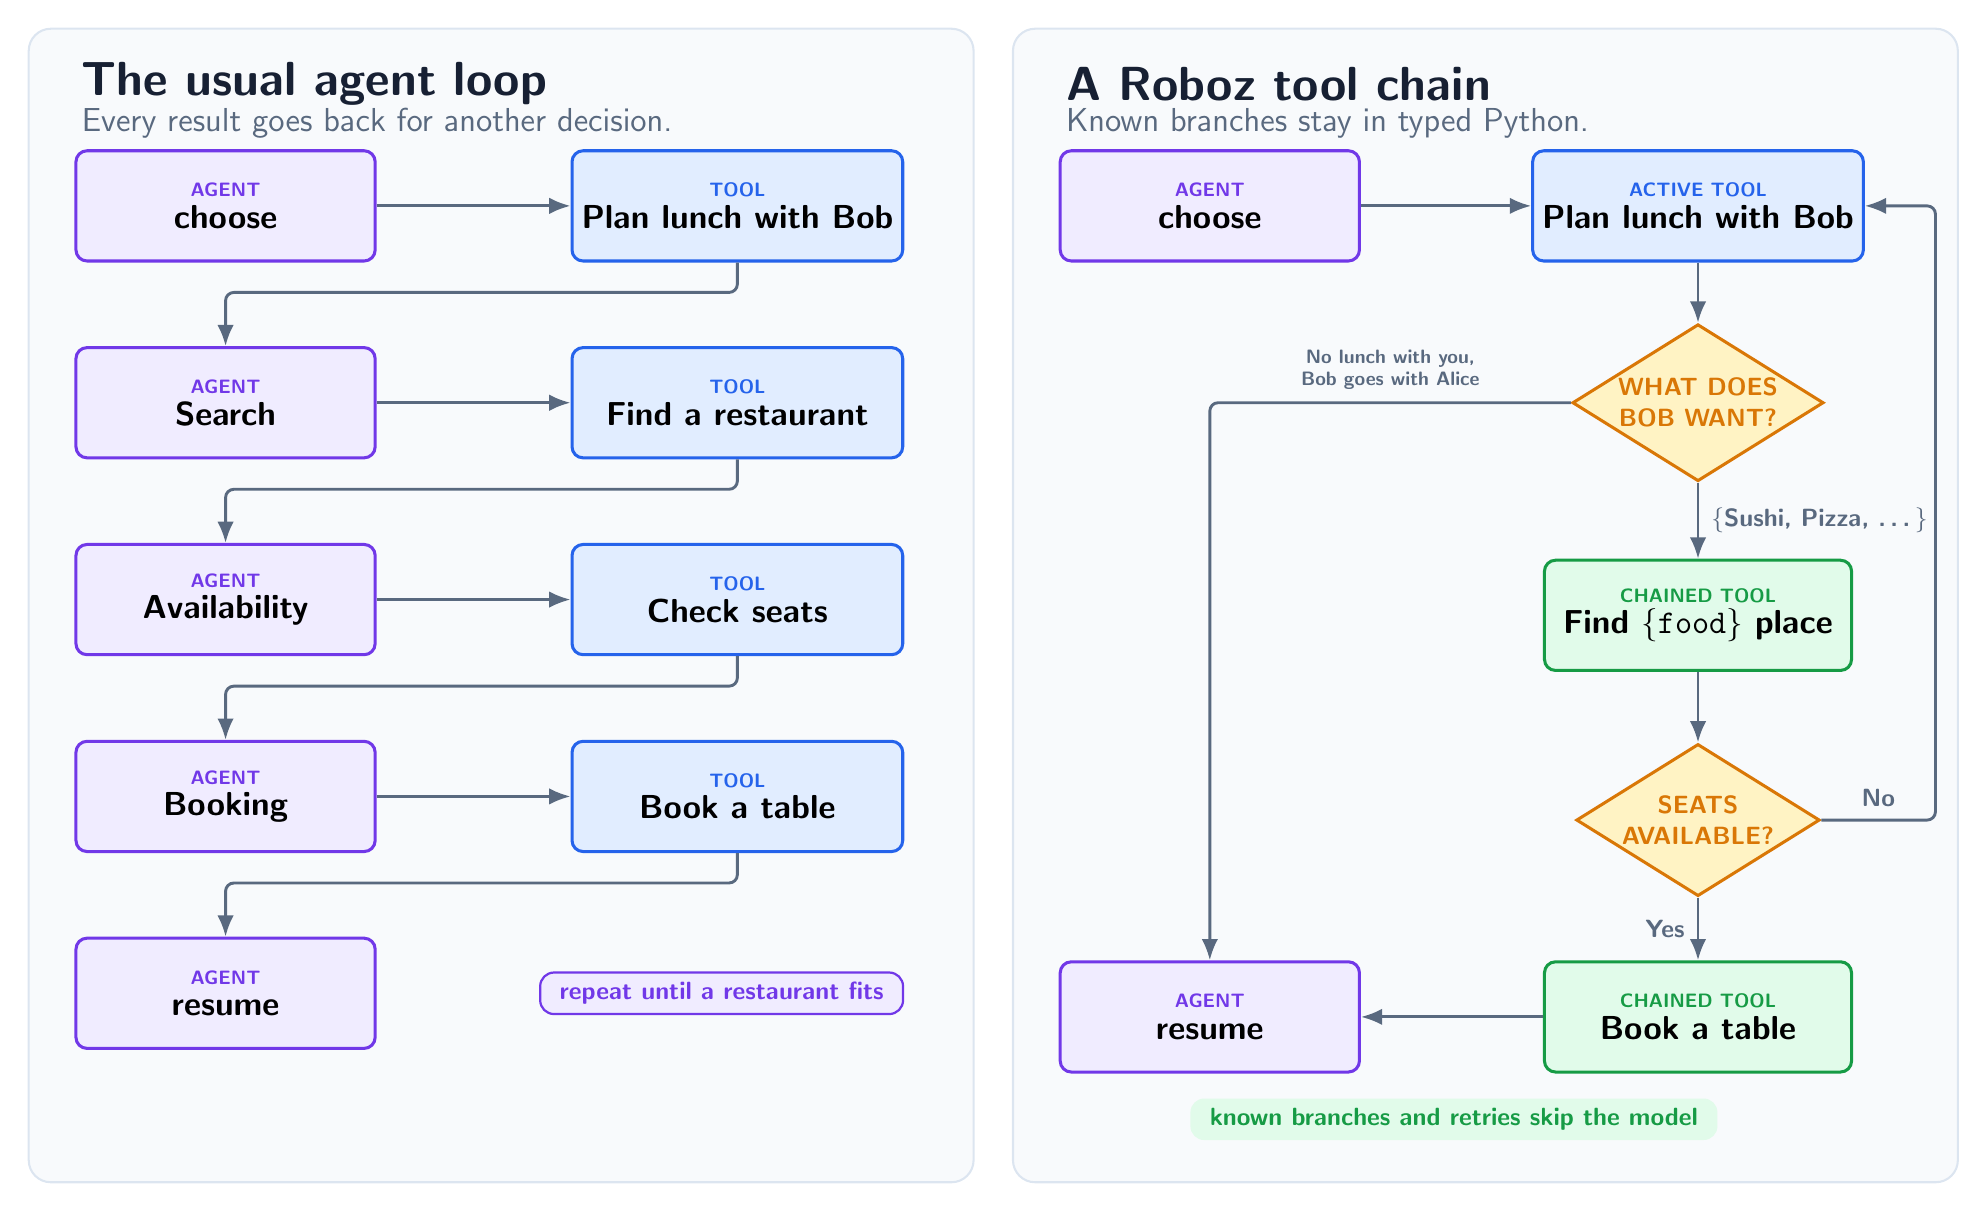
\begin{tikzpicture}[font=\sffamily]
  \begin{scope}[on background layer]
    \draw[draw=panelborder,fill=panel,line width=0.75pt,rounded corners=8pt]
      (-2,2.25) rectangle (10,-12.4);
    \draw[draw=panelborder,fill=panel,line width=0.75pt,rounded corners=8pt]
      (10.5,2.25) rectangle (22.5,-12.4);
  \end{scope}

  \node[anchor=west,font=\sffamily\bfseries\LARGE,text=ink]
    at (-1.45,1.55) {The usual agent loop};
  \node[anchor=west,font=\sffamily\large,text=muted]
    at (-1.45,1.05) {Every result goes back for another decision.};

  \node[agent] (loop-agent-1) at (0.5,0) {
    {\scriptsize\bfseries\color{purple}AGENT}\\[-0.2mm]
    {\large\bfseries choose}
  };
  \node[tool] (loop-tool-1) at (7,0) {
    {\scriptsize\bfseries\color{blue}TOOL}\\[-0.2mm]
    {\large\bfseries Plan lunch with Bob}
  };
  \node[agent] (loop-agent-2) at (0.5,-2.5) {
    {\scriptsize\bfseries\color{purple}AGENT}\\[-0.2mm]
    {\large\bfseries Search}
  };
  \node[tool] (loop-tool-2) at (7,-2.5) {
    {\scriptsize\bfseries\color{blue}TOOL}\\[-0.2mm]
    {\large\bfseries Find a restaurant}
  };
  \node[agent] (loop-agent-3) at (0.5,-5) {
    {\scriptsize\bfseries\color{purple}AGENT}\\[-0.2mm]
    {\large\bfseries Availability}
  };
  \node[tool] (loop-tool-3) at (7,-5) {
    {\scriptsize\bfseries\color{blue}TOOL}\\[-0.2mm]
    {\large\bfseries Check seats}
  };
  \node[agent] (loop-agent-4) at (0.5,-7.5) {
    {\scriptsize\bfseries\color{purple}AGENT}\\[-0.2mm]
    {\large\bfseries Booking}
  };
  \node[tool] (loop-tool-4) at (7,-7.5) {
    {\scriptsize\bfseries\color{blue}TOOL}\\[-0.2mm]
    {\large\bfseries Book a table}
  };
  \node[agent] (loop-resume) at (0.5,-10) {
    {\scriptsize\bfseries\color{purple}AGENT}\\[-0.2mm]
    {\large\bfseries resume}
  };
  \node[loop note] at (6.8,-10) {
    repeat until a restaurant fits
  };

  \draw[flow] (loop-agent-1) -- (loop-tool-1);
  \draw[flow] (loop-tool-1.south) -- ++(0,-0.38) -| (loop-agent-2.north);
  \draw[flow] (loop-agent-2) -- (loop-tool-2);
  \draw[flow] (loop-tool-2.south) -- ++(0,-0.38) -| (loop-agent-3.north);
  \draw[flow] (loop-agent-3) -- (loop-tool-3);
  \draw[flow] (loop-tool-3.south) -- ++(0,-0.38) -| (loop-agent-4.north);
  \draw[flow] (loop-agent-4) -- (loop-tool-4);
  \draw[flow] (loop-tool-4.south) -- ++(0,-0.38) -| (loop-resume.north);

  \node[anchor=west,font=\sffamily\bfseries\LARGE,text=ink]
    at (11.05,1.55) {A Roboz tool chain};
  \node[anchor=west,font=\sffamily\large,text=muted]
    at (11.05,1.05) {Known branches stay in typed Python.};

  \node[agent] (chain-agent) at (13,0) {
    {\scriptsize\bfseries\color{purple}AGENT}\\[-0.2mm]
    {\large\bfseries choose}
  };
  \node[tool] (chain-plan) at (19.2,0) {
    {\scriptsize\bfseries\color{blue}ACTIVE TOOL}\\[-0.2mm]
    {\large\bfseries Plan lunch with Bob}
  };
  \node[decision] (chain-food) at (19.2,-2.5) {
    {\small\bfseries\color{amber}WHAT DOES}\\[-0.3mm]
    {\small\bfseries\color{amber}BOB WANT?}
  };
  \node[passive] (chain-find) at (19.2,-5.2) {
    {\scriptsize\bfseries\color{green}CHAINED TOOL}\\[-0.2mm]
    {\large\bfseries Find \texttt{\{food\}} place}
  };
  \node[decision] (chain-seats) at (19.2,-7.8) {
    {\small\bfseries\color{amber}SEATS}\\[-0.3mm]
    {\small\bfseries\color{amber}AVAILABLE?}
  };
  \node[agent] (chain-resume) at (13,-10.3) {
    {\scriptsize\bfseries\color{purple}AGENT}\\[-0.2mm]
    {\large\bfseries resume}
  };
  \node[passive] (chain-book) at (19.2,-10.3) {
    {\scriptsize\bfseries\color{green}CHAINED TOOL}\\[-0.2mm]
    {\large\bfseries Book a table}
  };
  \node[note] at (16.1,-11.6) {
    known branches and retries skip the model
  };

  \draw[flow] (chain-agent) -- (chain-plan);
  \draw[flow] (chain-plan.south) -- (chain-food.north);
  \draw[flow] (chain-food.west) --
    node[
      edge label,
      above=0.8mm,
      pos=0.5,
      align=center,
      font=\sffamily\bfseries\scriptsize
    ] {No lunch with you,\\Bob goes with Alice}
    (13,-2.5) -- (chain-resume.north);
  \draw[flow] (chain-food.south) --
    node[edge label,right=0.8mm] {\{Sushi, Pizza, \ldots\}}
    (chain-find.north);
  \draw[flow] (chain-find.south) -- (chain-seats.north);
  \draw[flow] (chain-seats.east) --
    node[edge label,above=0.8mm] {No} ++(1.45,0) |-
    (chain-plan.east);
  \draw[flow] (chain-seats.south) --
    node[edge label,left=0.8mm] {Yes} (chain-book.north);
  \draw[flow] (chain-book.west) -- (chain-resume.east);
\end{tikzpicture}
\end{document}
